\section{Architecture and Design}\label{sec:archdesign}

\subsection{Architecture}
\begin{framed}
3. Use your design methodology found in 1. to describe a SysML/UML model of your system in terms of structure and behavior. Make a suggestion for alternative HW/SW architectures. Decide on which parts of the functionality should be mapped to hardware components and software processes.
\end{framed}

The overall structure of the system can be seen in the BDD in figure \ref{fig:bdd}. Here it can be seen, that the system should consist of three parts: \emph{User Interface}, \emph{Generation Generator}, and \emph{Simulator}. Each of the blocks has its own responsibility. 

\emph{User Interface} is responsible for getting the input from and to the user, e.g. the start generation and the final generation and fitness. 

\emph{Generation Generator} is responsible for generating the new generation using the genetic algorithm. \emph{Simulator} is responsible for calculating the fintness, i.e. the Rosenbrock function.

\begin{figure}[htbp]
\begin{centering}
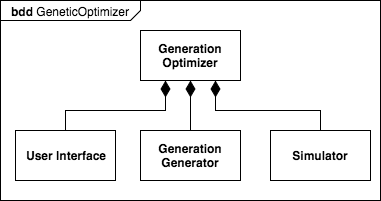
\includegraphics[width=0.7\linewidth]{../diagrams/bdd.png}
\caption{BDD of the system.}
\label{fig:bdd}
\end{centering}
\end{figure}

The internal connections can be seen in the IBD in figure \ref{fig:ibd}. The IBD shows a greater insight into which components are needed. It can be seen that \emph{GenerationGenerator} consists of two different parts, a generator and an interpreter of the random numbers. The point of the interpreter of the random numbers is, that it buffers the numbers such that there is always an amount of random numbers available.

\begin{figure}[htbp]
\begin{centering}
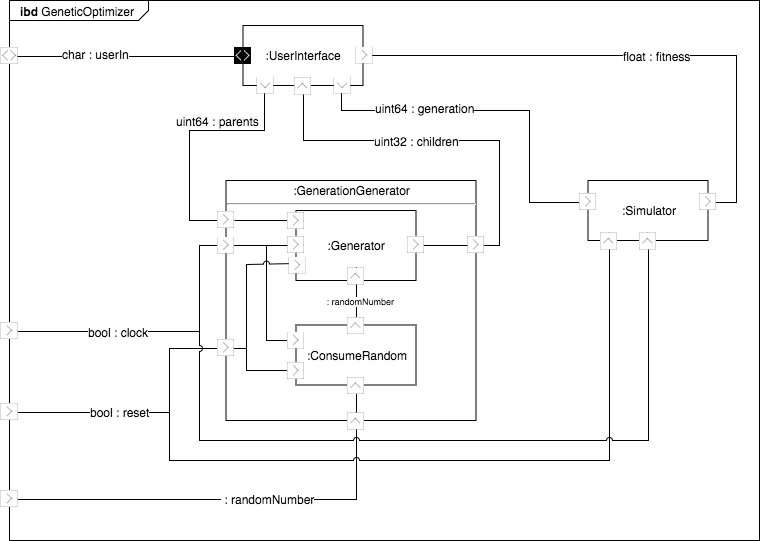
\includegraphics[width=\linewidth]{../diagrams/ibd.png}
\caption{IBD of the system.}
\label{fig:ibd}
\end{centering}
\end{figure}

The behavior of the system can be shown by activity diagram. This can be seen in figure \ref{fig:activity}, where the different elements of the system is described. It shows, that the user starts by setting some parameters and then initializes the initial generation. Then the initial generation is evaluated. If the stopping criterions, which can be set by the user, is met the final generation is saved and then it starts over. If the stopping criterion is not met GenerationGenerator generates a new generation and mutates it, as described in section \ref{sec:theory}.For each generation the fitness is printed out for the user. Then the fitness is evaluated, seen if the stopping criterion is met, and so on until the stopping criterion is met.

\begin{figure}[htbp]
\begin{centering}
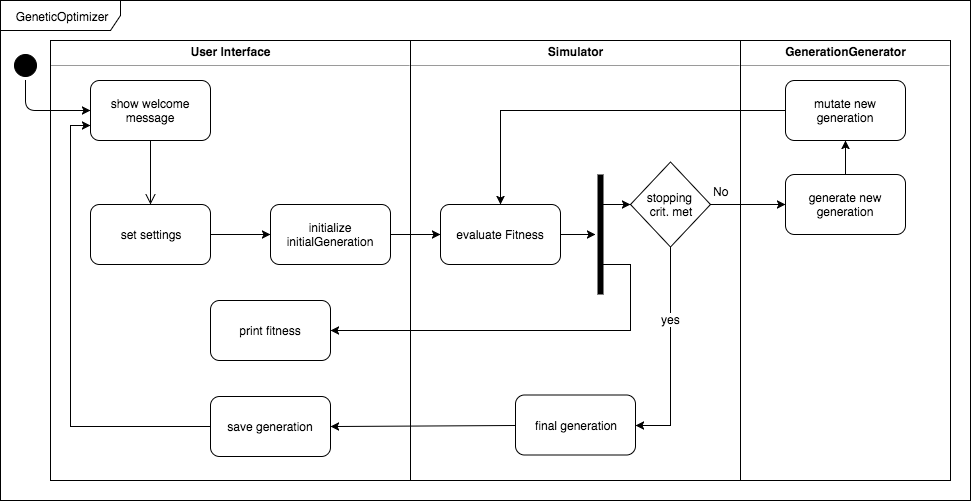
\includegraphics[width=0.9\linewidth]{../diagrams/overallActivity.png}
\caption{Activity diagram for the system.}
\label{fig:activity}
\end{centering}
\end{figure}

\subsection{Allocation}\label{sec:allocation}
The system has a number of possible allocations. A possible allocation is shown in figure \ref{fig:allocation}, which shows an allocation of both GenerationGenerator and Simulator to hardware. The user interface should not be allocated to hardware.

Other possible allocations are: \begin{itemize} 
\item Both GenerationGenerator and Simulator to software (the ARM processor).
\item GenerationGenerator to hardware (FPGA) and Simulator to software (the ARM processor).
\item GenerationGenerator to software (the ARM processor) and Simulator to hardware (FPGA).
\end{itemize}

As stated earlier it is needed that the generation of a new generation and the simulation should run in real-rime. This means, that, it is interesting to look at accelerating these parts using hardware, and use the allocation shown in the allocation diagram in figure \ref{fig:allocation}.

\begin{figure}[htbp]
\begin{centering}
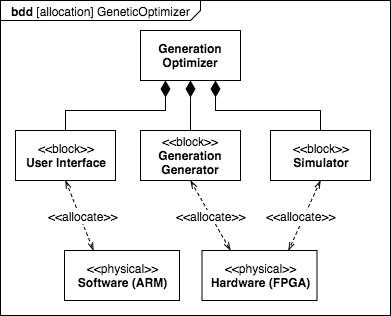
\includegraphics[width=0.9\linewidth]{../diagrams/allocation.png}
\caption{Allocation diagram of a possible allocation of the system.}
\label{fig:allocation}
\end{centering}
\end{figure}

\subsection{Design}
\begin{framed}
4. Design the software and apply design patterns that are suitable for your project, and motivate the choice of the used patterns. Use the Two-Part Architecture Model if relevant for the problem. Use the abstract OS package for the ZYBO board
\end{framed}

The software is designed using, mostly, the GoF Concurrent state pattern with events for changing states  using the command pattern.

The state machine for this can be seen in figure \ref{fig:statemachine}. Here it can be seen that there is two concurrent states. One is for loading random numbers in all the time and the other is the optimizer.

The only responsibility of the state for loading random numbers is to load random numbers and, when needed, pass them on to the generator.

The other state is a bit bigger. It consists of four different states where one is a nested state with two additional states. 
The states changes are triggered by the commands specified in the trigger in the state machine diagram in figure \ref{fig:statemachine}.

The state \emph{Idle} is a waiting state which the software is in when it enters and when an optimization is done or aborted or when it is done with a setup.

The \emph{Save} state is used to save the generation which has been optimized. This is done using a simple print to the terminal. 

\emph{Setup} is the state where the user is able to set the parameters $a$,$b$,the stopping criterions, and the initial generation.

The \emph{Optimize} is the nested state machine. This nested state machine is where most of the calculations happen. It starts in the state \emph{Simulate} where it finds the fitness of the generation. When the simulation is done it changes to either \emph{Idle} or \emph{GenerateGeneration} depending on whether the stopping criterions are met or not. It continues inside these until it has stopped or until it is aborted.

\begin{figure}[htbp]
\begin{centering}
\includegraphics[width=0.9\linewidth]{../diagrams/statemachine.png}
\caption{Statemachine diagram for the software.}
\label{fig:statemachine}
\end{centering}
\end{figure}

For implementing the concurrency the given OS abstraction library is used. This is a wrapper for the functions in FreeRTOS.


